%% Author: Mark weinreuter
\newcommand*{\VorlagenPfad}{../../Vorlagen}%
\documentclass{\VorlagenPfad/coderdojokatext}

% Titel, Kategorie müssen als Kommando für den Header/Footer definiert werden.
\newcommand{\Titel}{if-Abfragen}
\newcommand{\Kategorie}{Basics:\space} 

\begin{document}



\begin{center}
	{\huge \Titel}
\end{center}

\section{Entscheidungen und Bedingungen}
An vielen Stellen im täglichen Leben, sowie auch beim Programmieren müssen Entscheidungen getroffen werden:
'Soll ich früher aufstehen, um ihn Ruhe zu früchstücken oder lass ich das Frühstück ausfallen, damit ich länger schlafen kann?'
	
Um nun abends den Wecker zu stellen muss man sich Folgendes überlegen und ausführen:


\begin{pseudocode}
Falls <Will ich frühstücken?>:
	stelle_wecker(6)
Ansonsten:
	stelle_wecker(7)
\end{pseudocode}

Die Weckzeit ist also abhängig von der Bedingung: 'Will ich frühstücken?'.

\paragraph{Bedingung} Eine Bedingung beim Programmieren ist eine Aussage oder ein Ausdruck,
die mit 'Ja' oder 'Nein' zu beantworten ist. Komplizierte Antworten gibt es nicht! Eine Antwort
muss immer 'Ja' oder 'Nein' sein, 'Vielleicht' oder 'Morgen' sind nicht erlaubt.
\\
Um genau zu sein heißen diese Werte beim Programmieren meistens \code{True} (engl. für 'Wahr') und \code{False} (engl. für 'Falsch').
\\
Vielleicht stellst Du Dir jetzt die Frage, wie eine Bedingung zu formulieren ist, da 'Will ich frühstücken?' für Menschen einfach zu verstehen ist, für einen Computer allerdings nicht.

\paragraph{Die einfachste Bedinung} ist \code{True}('Wahr') oder \code{False} ('Falsch') zu schreiben.
\begin{pseudocode}
Falls <Wahr>:
	sage("Die Bedingung ist wahr")
\end{pseudocode}
Zugebenermaßen ist dies nicht sinnvoll, da man in dem obigen Beispiel die Bedingung einfach weglassen kann.
	
\paragraph{Vergleichsoperationen} sind eine Möglichkeit um Bedingungen zu beschreiben. Wie in der Schule können z.B. Operationen wie \code{>} (größer), \code{<} (kleiner),\code{>=} (größer gleich), \code{<=} (kleiner gleich) verwendet werden um Zahlen zu vergleichen.
\\
\\
Ein Ausdruck wie \code{30 > 20} ergibt \code{True} und \code{30 < 20} ergibt \code{False.} Diese können also als Bedingung verwendet werden kann.

\begin{pseudocode}
# 'alter' ist eine zuvor definierte Variable
Falls alter > 10:
	sage("Du bist älter als 10")
\end{pseudocode}

\clearpage

\begin{table}[t,clr]
	\begin{center}
	\begin{tabular}{|l|l|l|l|}
		\hline
		Operation		& Befehl		   	& Beispiel			 				& Ausgabe\\ \hline\hline
		Größer         	& \textgreater  	& 20 \textgreater\space20  			& Falsch \\ \hline
		Größer Gleich  	& \textgreater= 	& 20 \textgreater= 20 				& Wahr   \\ \hline
		Kleiner        	& \textless     	& 10 \textless\space30				& Wahr   \\ \hline
		Kleiner Gleich	& \textless=    	& 10 \textless= 25	    			& Wahr   \\ \hline
		Gleichheit    	& ==            	& 10 == 10	            			& Wahr   \\ \hline
		Ungleichheit  	& !=            	& 10 != 10            				& Falsch \\ \hline
	\end{tabular}
	\caption{Vorhandene Vergleichsoperationen}
	\end{center}
\end{table}

\section{Aufgaben}
\begin{itemize}
	\item Was (\code{True} oder \code{False}) ergeben die folgenden Ausdrücke jeweils:
	\begin{itemize}
		\item 10 \textless\space 12:
		\item 12 \textless\space 10
		\item 15 != 15
		\item 20 \textgreater= 15
		\item 12 == 12
	\end{itemize}
	\item In der Variablen \code{Schuhgröße} steht die Schuhgröße einer Person.
	\\
	Schreibe eine Falls-Ansonsten-Abfrage, die ausgibt (benutze 'sage'), ob diese Person große Füße hat oder nicht. Große Füße bedeutet, dass die Schuhgröße größer als 42 ist.
\end{itemize}

\clearpage

\section{if-Abfrage (Falls-Abfrage)} Bisher haben wir in den Beispielen keinen 'echten' Code verwendet. Dies wollen wir jetzt ändern.
Eine 'Falls'-Abfrage sieht in Python so aus:

\begin{pythoncode}
# 'wert' ist eine zuvor definierte beliebige Zahl-Varible
if wert < 10:
	print("Kleiner 10.")
	
print("Nach if-Abfrage.")
\end{pythoncode}

Dazu schreibt man \code{if} (engl. für 'falls), dann die Bedingung gefolgt von einem Doppelpunkt ':'. Darunter eine oder mehrere eingerückte Zeilen.
\\
Die Einrückung (mit 4 Leerzeichen oder Tabulator-Taste) bedeutet, dass alles was eingerückt ist \textbf{genau dann} ausgeführt wird, wenn die Bedingung wahr ist.
\\
\\
Führt man dies nun aus mit den Werten \code{wert = 5} und \code{wert = 15} aus, verhält sich die Ausgabe unterschiedlich:
\begin{pythoncode}
# wert = 5
Kleiner 10.
Nach if-Abfrage.
\end{pythoncode}


\begin{pythoncode}
# wert = 15
Nach if-Abfrage.
\end{pythoncode}

Man sieht an den Beispielen, dass 'Kleiner 10.' nur dann ausgegeben wird, wenn der Wert kleiner als 10 ist. Die nichteingerückte Zeile darunter wird in beiden Fällen ausgeführt und dies führt dazu, dass 'Nach if-Abfrage.' immer ausgeben wird.


\paragraph{Falls-Ansonsten-Abfrage (if-else-Abfrage)} Ist die Bedingung in der 'Falls'-Abfrage falsch, so kann eine 'Ansonsten'-Abfrage (engl. 'else') hinzugefügt werden, die \textbf{genau dann} ausgeführt wird, wenn die Bedingung falsch ist.

\begin{pythoncode}
# 'wert' ist eine zuvor definierte beliebige Zahl-Varible
if wert < 10:
	print("Kleiner 10.")
else:
	print("Größer oder gleich 10.")

print("Nach if-Abfrage.")
\end{pythoncode}
Führt man dies nun aus mit den Werten \code{wert = 5} und \code{wert = 15} aus, verhält sich die Ausgabe wie folgt:
\begin{pseudocode}
# wert = 5
Kleiner 10.
Nach if-Abfrage.
\end{pseudocode}

\begin{pseudocode}
# wert = 15
Größer oder gleich 10.
Nach if-Abfrage.
\end{pseudocode}

\paragraph{In Scratch} würde das obige Beispiel dann so aussehen:
\\
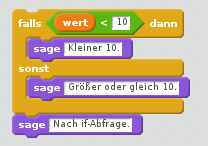
\includegraphics[scale=1]{scratch_if_else}
\\
Man sieht hier sehr schön die Einrückungen der 'sage'-Blöcke, während der grüne sptize Block die Bedingung darstellt.


\section{Aufgaben}
\begin{itemize}
	\item Du hast eine Variable 'zufall', die einen zufälligen Wert hat:
	\begin{pythoncode}
import random
zufall = random.randint(1, 100)
	\end{pythoncode}
	Schreibe eine if-else Abfrage die bestimmt, ob der Wert der Variablen größer oder gleich 50 ist oder nicht. Gib dies dann mithilfe des print() aus.
\end{itemize}

\end{document}